% Section content template for individual Educative lessons
% This file contains the actual content for a specific section
% Generated from Educative API section content

% Section: Getting Ready: The LinkedIn System
% Section ID: 5121032991277056
% Section Slug: getting-ready-the-linkedin-system
% Generated: 2025-12-14T13:33:48.118801

\subsection{Problem definition}\label{8t9y4PhhhzAHjxEhcwrhA}
\\
\textbf{LinkedIn} is a professional networking platform that helps users manage their professional identity. It enables users to connect with trusted professionals, grow their careers, and explore new opportunities.
\\
The platform enables individuals to create comprehensive professional profiles, featuring their education, experience, skills, achievements, and endorsements. Users can also create posts, interact with others' content, join or create groups, and manage connections.
\\
In addition to personal profiles, LinkedIn supports company pages, where organizations can list job openings and recruit candidates. Users can search for other professionals, send connection requests, exchange messages, and receive notifications about relevant activity.
\\
LinkedIn is very similar to Facebook in terms of its layout and design. However, its features are more specialized because it caters to professionals. If we are familiar with using Facebook or any similar social network, we may find LinkedIn familiar.

\begin{figure}[htbp]
 \centering
 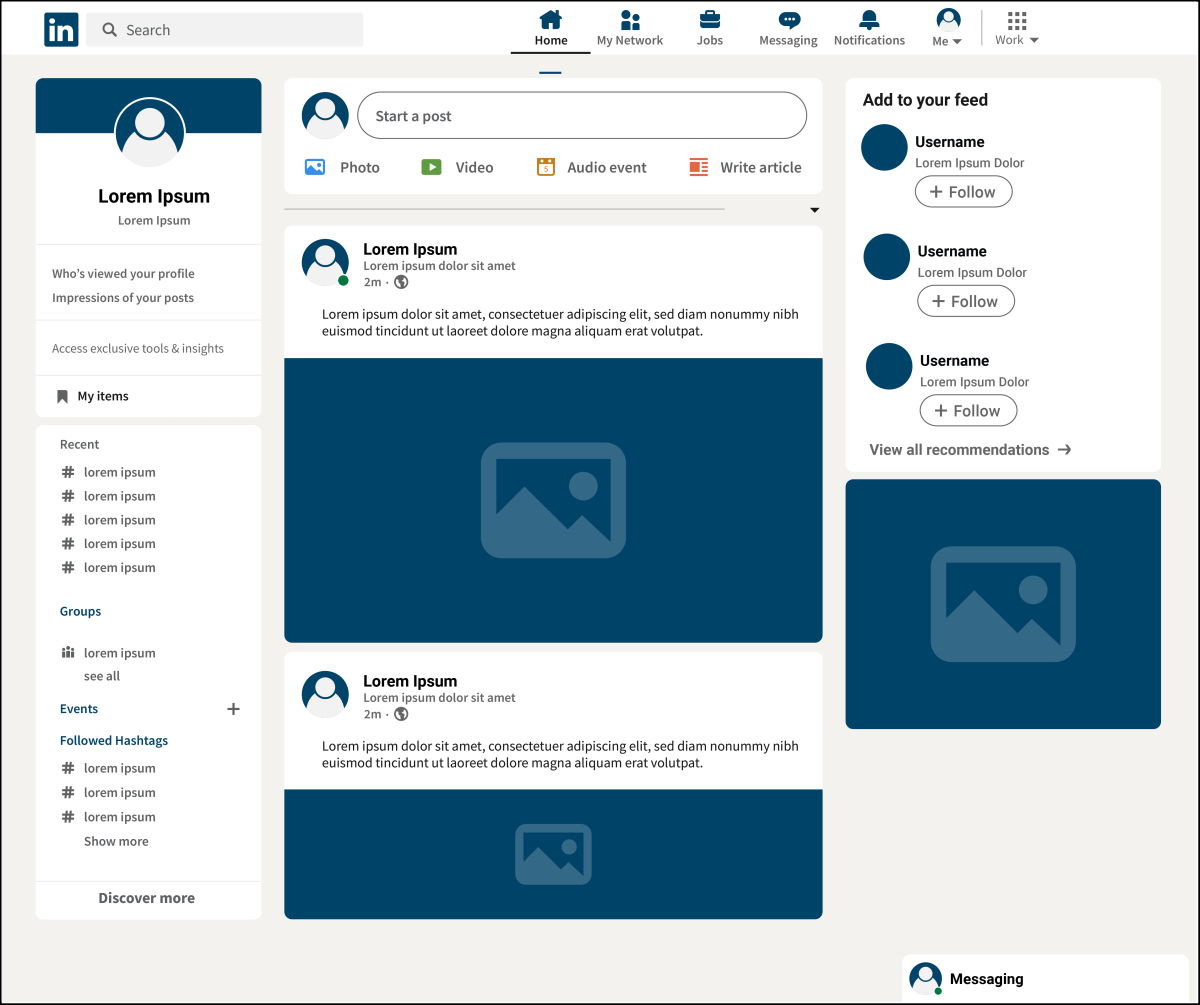
\includegraphics[width=0.5\textwidth]{Images/chapter_27/section_5121032991277056/6591997994598400.png}
 \caption{The home page of a LinkedIn user}
\end{figure}

\subsection{Expectations from the interviewee}\label{8mWjBBkzQ_msT38LKJm8y-2}
\\
LinkedIn offers a range of functionalities to its users. As our focus is limited to a specific set of features, it is essential to narrow down the components included in the LinkedIn design. The following sections highlight some key areas that the interviewer may expect you to explore during the system design discussion.

\subsubsection{Discoverability}\label{fKB2IFGj6alsP5vMPty6f}
\\
Understanding how users search for content and other users is important. The relevant questions include:

\begin{itemize}
\item
\protect\phantomsection\label{2J3pTA0h4L4bgYqMvsmZ0}
How are users able to search other users' profiles?
\item
\protect\phantomsection\label{A-9Zih7q5Rq_bECxVWCs5}
Can users search for groups and pages?
\end{itemize}

\subsubsection{Connections and following}\label{O0AvnObqEMkbA7isfb-Nz}
\\
Both connections and following are the primary features of LinkedIn. Make sure to ask the following questions of the interviewer:

\begin{itemize}
\item
How are users able to connect with other users?
\item
How can users follow or unfollow other users or company pages without needing to connect?
\end{itemize}

\subsubsection{Groups, pages, and jobs}\label{pqj0477HbElhoOwfLIuYF}
\\
Groups and pages on LinkedIn create a space for people looking for similar job opportunities. Make sure to define your requirements. You may ask the following questions of the interviewer:

\begin{itemize}
\item
\protect\phantomsection\label{1vUCXAfis_vqykq_q3HLI}
Can users create both groups and company pages?
\item
\protect\phantomsection\label{scw5UOrNkBVt5_5HTGDVZ}
Can users join a group?
\item
\protect\phantomsection\label{4k5m_VbmBbUeb9Nl1rfK-}
Can users follow company pages?
\item
\protect\phantomsection\label{JO_zEKrOom5mIQlMtjq_V}
Can company pages post jobs that users can apply for?
\end{itemize}

\subsubsection{Alerts}\label{zFvYTq0vpb5ZfVBAwB6W2}
\\
Notifications and alerts enable users to stay informed about activity within their circle. Therefore, you may want to understand how alerts work in your system. You may ask the following questions:

\begin{itemize}
\item
\protect\phantomsection\label{0hn0qGMWYin6fQ-OjCKaM}
How will users be notified about messages, connection requests, or comments on their posts?
\end{itemize}

\subsection{Design approach}\label{8SKp8Noe0yP0-ji5F2BPW}
\\
We'll follow a bottom-up design approach to build the LinkedIn system. The steps include:

\begin{itemize}
\item
Design the smallest units first (e.g., posts, comments, users, connections).
\item
Combine these to build larger components (e.g., groups, company pages, profiles).
\item
Continue layering until the complete LinkedIn platform is modeled.
\end{itemize}

\subsection{Design pattern~}\label{VD8QsBZg9_Th1KK6XiY9w}
\\
During an interview, it is always a good practice to discuss the design patterns that LinkedIn falls under. Stating the design patterns gives the interviewer a positive impression and shows that the interviewee is well-versed in the advanced concepts of object-oriented design.
\\
Try to answer the following question. If you are not familiar with design patterns, don't worry! You can learn about them by asking, ``Define design patterns.''

\textbf{Question:}

Which design pattern(s) should be used to design the LinkedIn system? Please elaborate on your choice(s).

.
\\
Let's explore the requirements of the LinkedIn design in the next lesson.

% End of section content